%!TEX root = ../../main.tex

% intro

\chapter[Introduction]{Introduction}
\label{thesis:intro}

In this first chapter, we give a primer on \emph{Reinforcement Learning},
abbreviated \textit{``RL''} throughout the thesis.
RL constitutes the common denominator of every research endeavors undertaken, reported, and
discussed at length in this thesis.
We lay out the foundations in this chapter, and will enrich this federating introduction,
at the beginning of each subsequent chapter, with additional introductory elements
in order for the reader to grasp how each of the treated settings branches out of RL.

The chapters of this thesis align with the contributions laid out in the following articles:
\begin{description}
\item[\textsc{Chapter}~\ref{thesis:chap1}]
Lionel Blondé, Alexandros Kalousis.
\textit{Sample-Efficient Imitation Learning via Generative Adversarial Nets.}
Presented at AISTATS (poster); Apr 2019; Naha, JP
\item[\textsc{Chapter}~\ref{thesis:chap2}]
Lionel Blondé, Strasser Pablo, Alexandros Kalousis.
\textit{Lipschitzness Is All You Need To Tame Off-policy Generative Adversarial Imitation Learning.}
Post-rebuttal at the MLJ 2021
\item[\textsc{Chapter}~\ref{thesis:chap3}]
Lionel Blondé, Alexandros Kalousis.
\textit{Where is the Grass Greener? Revisiting Generalized Policy Iteration for Offline Reinforcement Learning.}
To be submitted at the JMLR 2021
\end{description}

\section{RL in a nutshell}

Reinforcement learning is the field of
sequential decision making under uncertainty,
where the decision maker must learn to maximize its long-term utility
by interacting with a stateful world that rewards it with feedback upon interaction.
The world or \emph{environment} is unknown to the agent who can only learn from it through explicit
interactive queries.
Upon reacting to the agent's decision, the state of the world changes.
From a practitioner standpoint, one must design a learning procedure
that enables the decision maker to figure out how to best answer the following question:
\textbf{\emph{what decision rule should I adopt to act \emph{optimally} in any given situation?}}
An agent is deemed \emph{optimal} if its decision rule or \emph{policy} enables it to
accumulate more rewards in every episode of interaction
than any other strategy,
regardless of how the world reacted to each intermediary decision.
Rewards are often delayed, delivered to the agent only after it has already committed
to an interaction strategy.
Receiving a comparatively high reward at a given state of the multi-stage decision process does not
necessarily means that the action executed at said state was good,
it might instead be due to having made a good decision a few steps prior.
Identifying which decisions led to a satisfactory or disappointing outcome
--- equivalently, which actions \emph{deserve credit} for the perceived result --- is a tall order.
This challenge is known as the \emph{temporal credit assignment problem},
across naturalistic behavioral disciplines
\footnote{
The temporal credit assignment problem has first been addressed by \cite{Minsky1961-qb}
in an artificial intelligence context.
It was also studied, albeit later,
in a branch of experimental psychology focused on animal behavior processes sometimes
referred to as animal learning, \textit{e.g.} in \cite{Mackintosh1975-yg}.
Operant conditioning --- class of associative learning, and subfield of animal learning;
\textit{cf.} \cite{Skinner1948-nh} for an early work on- and \cite{Mackintosh1983-kd} for an account on
operant conditioning
---
have been shown to have a lot in common with RL,
\textit{e.g.} in \cite{Schmajuk1997-hq} and \cite{Touretzky1997-tm}.
Note, operant conditioning exposes the animal to \textit{reinforcers} (counterpart of RL's rewards)
depending on its \emph{decisions}, unlike Pavlovian (or classical) conditioning in which the animal's
behavior is \emph{not} reinforced \textit{w.r.t.} what it does
(\textit{cf.} Dickinson's animal learning book \cite{Dickinson1980-oq}).
Connections have also been made in neuroscience between RL's rewards and
dopamine neuron responses
(\textit{e.g.} \cite{Ljungberg1992-fr}, \cite{Montague1996-iy}, \cite{Schultz1997-xx}, \cite{Dabney2020-nm}).
}.

\section{An artificial agent in a Markovian world}

Facing the resolution of the reinforcement learning problem,
the decision maker or agent is set in an interactive world,
referred to as environment, and denoted by $\mathcal{E}$.
The environment $\mathcal{E}$ is modeled as a memoryless, infinite-horizon, and stationary
\emph{Markov Decision Process} (\textit{abbrv.} MDP), noted $\mathbb{M}$.
Formally, the MDP is defined as the tuple
$\mathbb{M} \coloneqq (\mathcal{S}, \mathcal{A}, p, \rho_0, u, \gamma)$, where
$\mathcal{S} \subseteq \mathbb{R}^n$ and $\mathcal{A} \subseteq \mathbb{R}^m$
are respectively the state space and action space of the MDP.
describing the states and actions that \textit{can} occur in the decision process.
Intuitively, states correspond to \emph{situations}, and actions to \emph{decisions}.
Due to the discrete-time structure of a MDP,
the experiences of the agent are divided across discrete timesteps $t$, or \emph{stages}, where $t\geq0$.
One may refer to any number of sources to get a comprehensive account on these multi-stage decision processes,
\textit{e.g.} \cite{Ross1983-oc} or \cite{Puterman1994-pf}.
Note, these books tackle \textit{finite} MDPs (FMDPs) for the most part,
defined as MDPs whose state and action spaces are both finite.
Due to their conceptual simplicity compared to their continuous alternative, FMDPs
have unsurprisingly been the object of far more studies.
Besides, as stressed by Sutton in \cite{Sutton1998-ow},
one generally need not look further that FMDPs
to deal with 90\% of modern reinforcement learning problems.

The \emph{dynamics} of the environment $\mathcal{E}$,
\textit{i.e.} how the Markovian world reacts to the agent's decisions,
are determined by both $p$ and $\rho_0$.
The initial state probability distribution is built from the associated density $\rho_0$, while
$p$ is the stationary and stochastic transition function that decides how the environment's MDP transitions from
one state to the next upon being affected by a decision from the agent.
In concrete terms, $p(s' | s, a)$ is the conditional probability density
concentrated at the (next) state $s'$ when action $a$ is executed in state $s$.
Upon transitioning from $s$ to $s'$ via the action $a$ in $\mathcal{E}$,
the agent from which $a$ originated is provided with feedback from $\mathcal{E}$,
called reinforcement signal, or simply reward.
The real-valued reward $r$ received by the agent in response to this interaction
is distributed as $r \sim u(\cdot | s, a)$, where $u$ is modeled as a stationary reward process.
Completing the $\mathbb{M}$ tuple,
the discount factor $\gamma$ is a coefficient that discounts the perceived payoff,
to be picked in the $[0, 1)$ real interval.
It remains frozen at the preset value throughout the learning process;
usually set at a value near $0.99$.

The decision maker behaves in line with what its policy $\pi$ dictates.
$\pi$ is followed consistently --- at every stage of the decision process,
and is modeled as a stochastic function that
maps states to probability distributions over actions, \textit{i.e.}
as $\pi : \mathcal{S} \to \mathcal{P}(\mathcal{A})$
(or as $\pi : \mathcal{S} \to \mathcal{A}$, if $\pi$ is chosen to be deterministic).
Concretely, at $s \in \mathcal{S}$, the agent
concentrates a probability density equal to
$\pi(a | s)$ at action $a \in \mathcal{A}$.
If $\pi$ puts a density $\pi(a | s)$ at $a$ every time $s$ is visited (whatever the stage),
then $\pi$ is said to be \emph{stationary}.

Rather than considering a \emph{finite}-horizon MDP,
the \emph{infinite}-horizon MDP setting is adopted.
As such, the state $t$ of the multi-stage process is \textit{a priori} unbounded above in the formalism.
Still, despite being within the infinite-horizon setting,
one can posit that every trace contains at least one absorbing state,
effectively making the MDP episodic.
The discount factor $\gamma$ is artificially set to zero when one such state is reached
in order to emulate termination, hence formally constructing an \textit{episode}.
This will become more apparent when discussing the concept of \emph{return}.
When the analyses carried out call for the involvement of a finite time horizon $T$,
how far the horizon is set will be adjusted accordingly.

The stateful interactive process between the agent and the environment is depicted
in \textsc{Figure}~\ref{fig:rl}.

\begin{figure}
\center
\scalebox{0.25}[0.25]{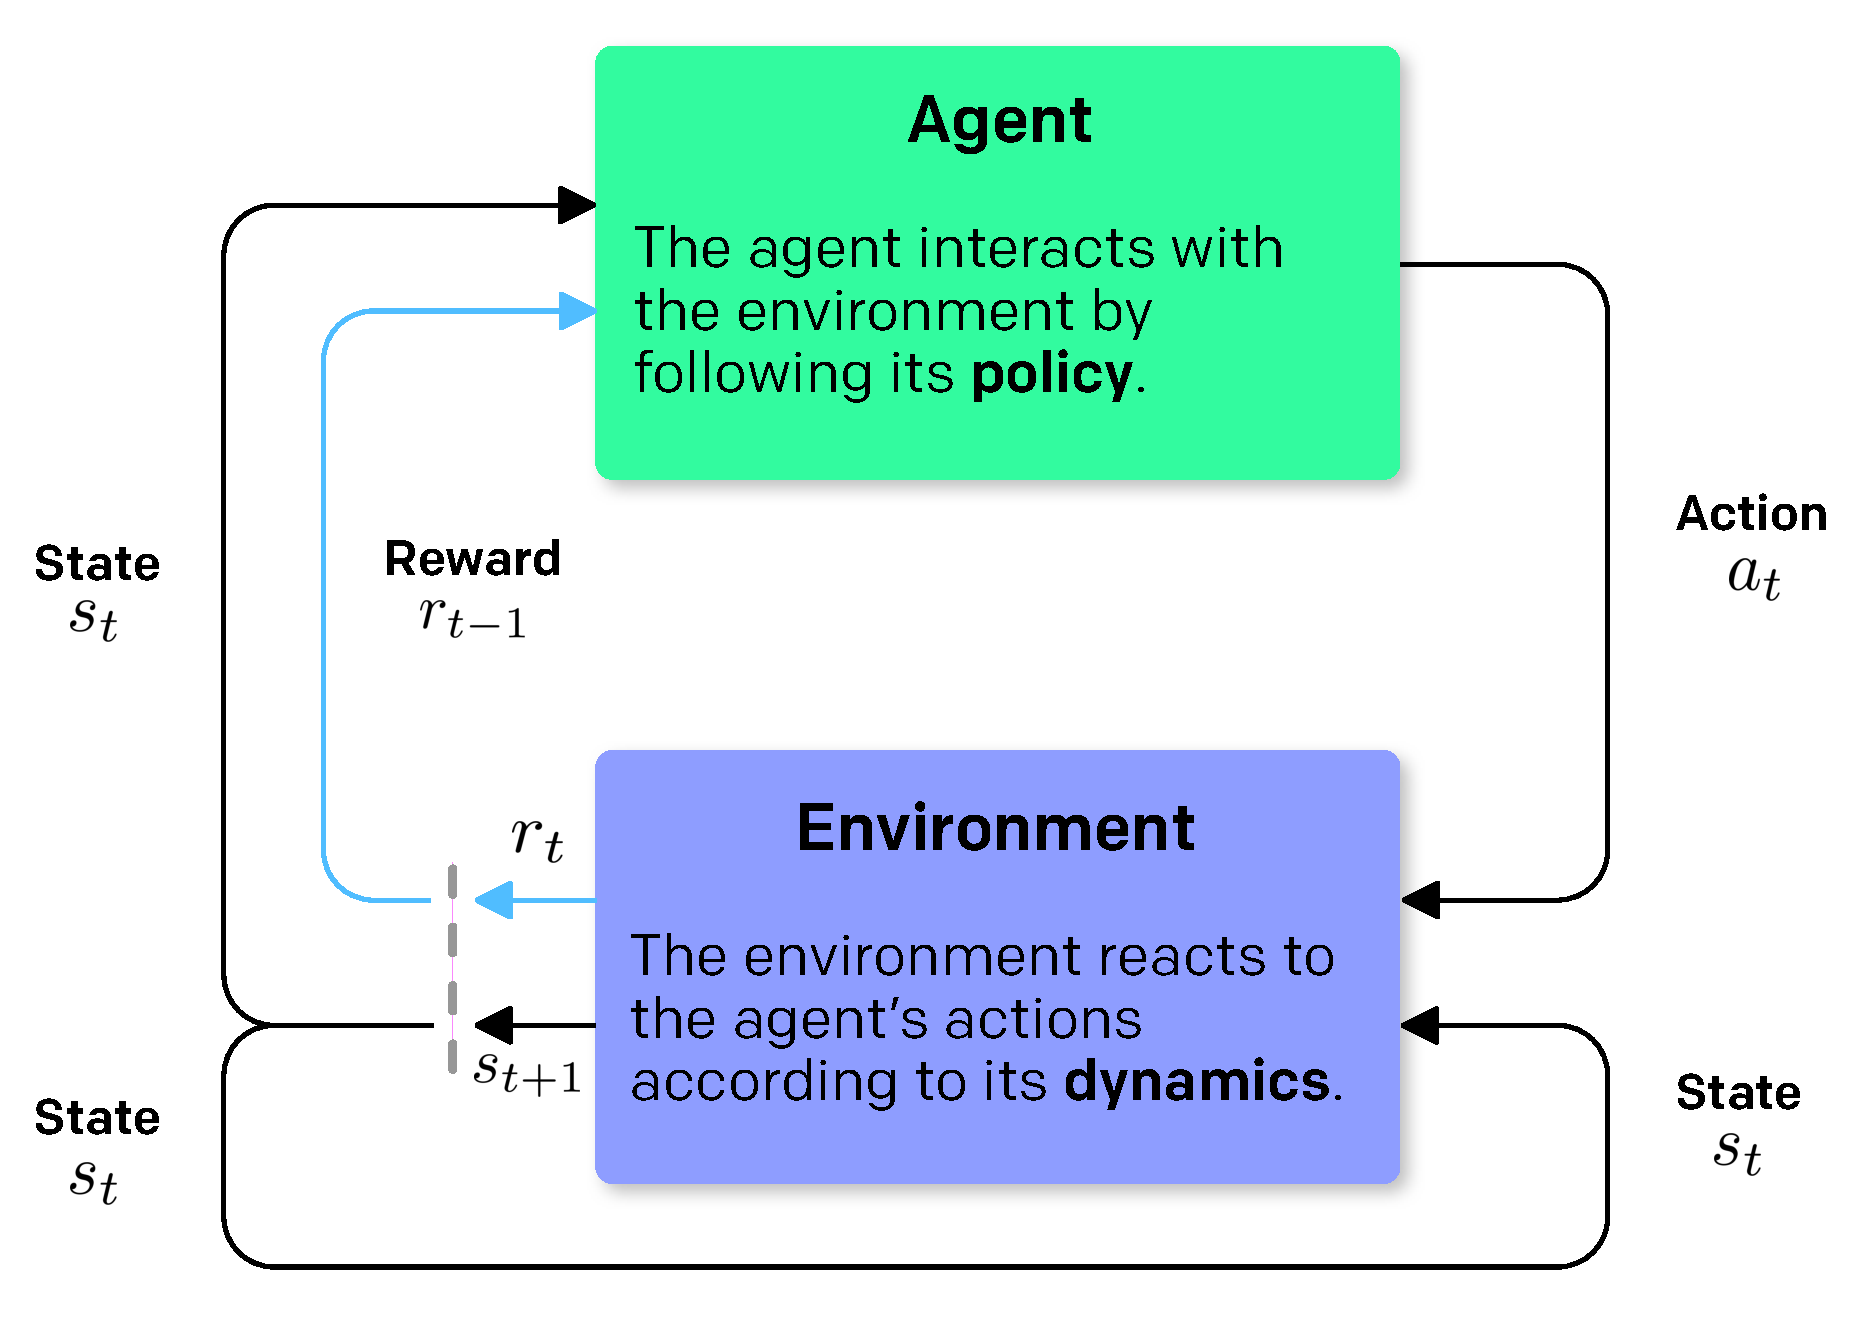
\includegraphics{Diags/rl}}
\caption{Reinforcement learning interaction diagram (similar to the one in \cite{Sutton1998-ow}.}
\label{fig:rl}
\end{figure}

For most of the theory developed in RL over the last decade to apply,
one must assume that the Markovian world satisfied the \emph{Markov property}.
More accurately, one must assume that the conceptual MDP used to model how the worlds
reactions to the agent's decision follows said property.
The latter is likely not a property verified by the \emph{real} world,
but one that we can assume for the model set over the environment to best
represent its inner workings and structure.
The Markov property states that all that can be deemed as relevant in the history of interaction
is present in the current state. Looking backwards at anything older that the current state would be redundant.
By relying on this property,
the decision maker can then base its current action solely on the current state,
and need neither use nor even know about the MDP's past.
As such, the transition and reward processes need
($p$ and $u$, respectively) depend only upon the state and the action from the \emph{current} stage,
and upon \emph{none} of the states and actions respectively occupied and executed by the agent at previous stages.
This explains the design choices made to model $\pi$, $p$, and $u$ in the paragraphs above.
The Markov property is well illustrated by Silver:
\textit{``the future is independent of the past given the present''}, in lecture \cite{Silver2015-wm}.

Reinforcement learning relies on the \emph{reward hypothesis},
stipulating that one can equivalently treat the satisfaction of a preset goal
as the maximization of an accumulation of perceived scalar rewards.
In line with this hypothesis, the completion of a task should coincide, from the agent's perspective,
with having reached the utmost cumulative amount of rewards achievable during its learning lifetime.
Adopting the practitioner's perspective,
the reward function must be purposely designed such that it aligns with the satisfaction of this desideratum,
both qualitatively (the agent must receive rewards when it does well)
and quantitatively (it must receive increasingly higher rewards as it gets better at solving the task).
Reward alignment is tedious to carry out, as rewards are easily prone to misspecification,
and therefore usually require an inordinate amount of trial-and-error prior experimentations,
going through handcrafted iterates of designs until it encodes the task properly, and instills the desired
behavior primitives into the agent.
This intensive iterative process is usually referred to as \textit{reward shaping},
for which \cite{Ng1999-lv} has been the reference.
For example, \cite{Randlov1998-qo} gives an account on how they managed to teach
an artificial agent how to drive a bicycle,
via reinforcement learning, yet through the extensive (albeit successful) use of reward shaping.
On the flip side, there have various reported occurrences of reward misalignment leading to
the unintended collapse of the agent onto another (usually trivial) task.
From the practitioner's standpoint, it might look like the agent is malevolently bypassing the task
it was asked to complete, while in effect, it merely was not able to understand the intent behind the
reward signal crafted purposely by the practitioner to induce the desired (unachieved) behavior.
Such a phenomenon has been aptly dubbed reward \textit{hacking}, or reward \textit{hijacking}, or
even reward \textit{corruption}, \textit{cf.} OpenAI's blog post \cite{Amodei2016-vg}
for an animated account on faulty reward function and companion paper \cite{Amodei2016-tb} for
guidelines and pointers on reward modelling.

A particularly striking occurrence of reward misspecification can be witnessed in
the biorobotics works lead by Taylor and reported in \cite{Hoyt1981-ma} and \cite{Farley1991-fd}.
Albeit separated by a ten-year gap, these works tackle the problem of identifying and understanding
what is the primary physiological signal whose optimization would best explain the observed kinematics
in horse gaits. First, based on their empirical findings, \cite{Hoyt1981-ma} claimed that animals (such as
the horses they studied) regulate the speed at which they switch gaits such that it minimizes the energy costs
provoked by the change of gait.
It was later disproved in \cite{Farley1991-fd} who showed that natural occurrences of gait switches can
be accompanied with higher energy consumption. Instead, it was reported that transitions occur once
musculoskeletal forces put muscles, tendons, or bones under critical strain.
Avoiding chances of injury then seemed to be what physiologically determined the speed at which horses switch gait,
not the energetic cost of the switch.
This line of work showcases that solving the inverse problem of identifying
\textit{what is the signal that, when optimized, would explain the observed behavior}
(exactly what \emph{inverse} reinforcement learning, or IRL, aims to solve)
is a tall order.
One must therefore be cautious when it comes to specifying rewards to induce a certain behavior,
as one's intuitions (sometimes backed by published research) about the inverse problem
--- what is the objective (reward) that is being optimized by the actor displaying the observed behavior ---
might be off track,
leading to fatally erroneous specifications.
In the abstract \cite{Russell1998-yk},
Russell also draws a parallel between reinforcement learning and econometrics,
noticing that the inverse problem of RL has been tackled
by econometricians
as the problem referred to as \textit{structural estimation of Markov decision processes},
of which \cite{Rust1994-iw} gives an account in 1994.


Reward design constitutes an active subfield of reinforcement learning research.
The research endeavors reported in
both \textsc{Chapter}~\ref{thesis:chap1} and \textsc{Chapter}~\ref{thesis:chap2}
tackle the problem of \emph{learning} reward functions in the context of imitation learning ---
drawing stronger ties with inverse reinforcement learning and apprenticeship learning specifically,
thereby avoiding the burden of manual reward shaping.

Making the agent decide what decision to make at the current state \emph{solely} so as to
maximize the \emph{immediate} reward is far from ideal, since rewards can be delayed
(\textit{cf.} Watkins' thesis, \textit{``Learning from Delayed Rewards''}).
The agent's decision or action for the current state might only reveal itself as good at a later stage,
even if not immediately rewarding at execution.
An action that appears non-rewarding now might lead to areas of the state space where the decisions made by
the agent would \emph{then} yield high rewards, even it very few rewards have been perceived along the way
--- hence, \textit{``delay''}.

Instead, it is far better for the decision maker
to maximize the rewards it gets and will get
\textbf{\emph{in every stage from the current one to the end of the episode}},
\textit{i.e.} over \textbf{\emph{current and future}} stages.
In order to formally account for these future rewards, albeit unoccurred at the current stage,
the can maximize the entity dubbed \emph{return}, defined here as the
discounted sum of future rewards (including the immediate reward received upon execution of the current action).
While several alternative definitions of the return have been proposed and studied in prior art
(\textit{e.g.} average reward, undiscounted sum of future rewards),
we stick to the discounted total sum of rewards mainly due to its widespread usage,
but also due to its convenient analytical behavior in the infinite-horizon setting.
The \textit{discount} in question for the considered return variant
is determined by the discount factor $0 \leq \gamma < 1$ introduced earlier.
Consider the reward $r_t$ as being the reward received by the agent upon acting at stage $t$.
In the adopted discounted infinite-horizon setting,
the return $R_t^\gamma$ of the agent at stage $t$ is,
$\forall t \in \mathbb{N}$:
\begin{align}
R_t^\gamma
\coloneqq
\sum_{k=0}^{+\infty} \gamma^k r_{t+k}
= r_t + \gamma r_{t+1} + \gamma^2 r_{t+2} + \gamma^3 r_{t+3} + \cdots + \gamma^u r_{t+u} +\cdots
\label{intro:returndef}
\end{align}
Note, if one were to use a \emph{finite} horizon $T$, the return at $T$ would coincide with the reward at $T$
since there is no future to account for, no future rewards to assess,
and nothing to discount: $R_T^\gamma = r_T$.
To get a grasp on the extent to which future rewards are discounted as we step further into the future,
consider a discount factor $\gamma=0.99$. With such a $\gamma$ value,
$r_{t+1}$ is discounted by a factor $\gamma=0.99$,
$r_{t+2}$ by $\gamma^2 \approx 0.98$,
$r_{t+50}$ by $\gamma^{50} \approx 0.61$,
$r_{t+100}$ by $\gamma^{100} \approx 0.37$,
$r_{t+200}$ by $\gamma^{200} \approx 0.14$,
$r_{t+500}$ by $\gamma^{500} \approx 0.0066$.
In other words, with $\gamma=0.99$, the return $R_t^\gamma$ effectively neglects the rewards
the rewards received by the agent past $500$ steps into the future starting from $t$.
By contrast, when picking a higher discount factor, \textit{i.e.} $\gamma=0.995$,
$r_{t+500}$ is then only discounted by a factor of $\gamma^{500} \approx 0.082$.
The closer $\gamma$ is to $1$, the further $R_t^\gamma$ can \emph{propagate} rewards
backwards, along the chain of decisions, from stage $t+u$ to stage $t$,
\textit{i.e.} handle greater delays in rewards. $\gamma$ determines from how far into the future the agent
can propagate rewards to the current stage.
Picking a greater $\gamma$ nevertheless comes at the cost of being exposed to a harder credit assignment
--- \textit{backward reward propagation} being the latest refinement of this problem ---
since the effective horizon is larger
(less discount from one stage to the next).
\textit{In fine}, if $\gamma=0$, the return trivially collapses onto the immediate reward,
($R_t^\gamma = r_t$), a case of little interest.

The aims for the RL agent is then to find an \emph{optimal} policy to follow --- noted $\pi^*$, where
\emph{optimality} aligns with the ability of $\pi^*$ to always collect the maximum achievable return
$R_t^\gamma$ for every stage $t$.
Wherever the decision maker starts, it will always pick the best action in terms of long-term gains.
To instill such an optimal behavior into the agent, one must be able to identify what are the actions
executed in the course of a given episode by the decision maker that most \emph{deserve} to be given credit.
The concept of return naturally plays an instrumental role in determining which are responsible for allowing the
agent to be rewarded for its performance at progressing towards task completion, albeit with a delay.
This problem of knowing who to assign credit to or who to blame
in the context of a sequential decision process
is known as the \emph{(temporal) credit assignment problem}, and the notion of return is at the center
of its resolution.
By definition, optimal policies --- non-unique \textit{a priori}; unicity of optimality in policy space
discussed momentarily --- solve the temporal credit assignment problem, and as such, are the ones
one must teach one's RL agent how to search for.
\emph{Where should the one look for to find an optimal policy?}
As shown by Ross in \cite{Ross1983-oc},
in every FMDP, among all the optimal policies,
there exists at least one optimal policy that is stationary and deterministic
--- \textit{stationarity} (or time-homogeneous; defined earlier)
for deterministic policies signifies that the agent always picks the \emph{same}
action whenever it faces the same state.
Since there exists a deterministic stationary policy that is optimal (proven by Ross in a \emph{F}MDP),
and since verifying these two properties is \textit{a priori} more appealing than the alternative,
it is generally-speaking a good idea for the agent to search for an optimal policy \emph{solely} in the
space of stationary deterministic policies.
Concretely, determinism is naturally modeled via a functional mapping without probabilistic sampling unit of any
kind, and the added stationarity can be urged by learning a \emph{single}
deterministic policy for all states and for all stages.
Learning one distinct policy \emph{per stage in the episode} would result in a \textit{non}-stationary
(or time-heterogeneous) policy, which are far more tedious to learn in terms of compute and implementation costs.
As such, one usually leverages the previous theoretical results first articulated by Ross,
and set out to look for an optimal policy in the space of stationary deterministic policies,
whose existence has been proved in FMDPs.
Puterman enriches the theoretical results of Ross by a considerable margin in \cite{Puterman1994-pf}.

\section{How to solve the temporal credit assignment problem?}

Now that we have established that temporal credit assignment in multi-stage decision processes
is the problem that the interactive agent must solve to carry out its assigned task optimally,
we need answer the following:
\textbf{\emph{How should one go about solving the (temporal) credit assignment problem?}}
Historically, there have been two main methods, both spanning their own respective collection of algorithms,
that have aimed at figuring out how to assign credit to decisions sequentially made by artificial agents over time.
Whether there is actual interaction with the Markovian world as the optimal strategy is sought after is
conceptually outside the scope of this investigation at least at the level of granularity we target here).
These two wide-ranging methods are \textit{1)} dynamic programming and
\textit{2)} reinforcement learning (the one we focus on in this thesis).
There is a considerable overlap between the two approaches to assigning credit in time,
as both are built upon the same principle of optimality to derive optimal behavior primitives.
Said principle of optimality will be laid out momentarily.

Albeit constructed from the same foundational basis to craft agents that act optimally,
the two approaches and the algorithms that follow their respective paradigms differ by what they assume
is known about the world, and therefore what they are allowed to leverage from this knowledge.
Not to be mistaken for its computer science counterpart
(although its underlying, defining pattern of \textit{overlapping sub-problems}
fits the considered control theory interpretation too),
dynamic programming \emph{need} access to a perfect model of the environment.
Besides, the latter need be modeled as a MDP,
which concretely allows the artificial agent to evaluate the probability of a transition $(s,a \to s')$
to occur by having access to $p$, or the probability of receiving the reward $r$ upon executing $a$ in $s$
by being also granted access to $u$ from the decision process,
$\forall \, s, s' \in \mathcal{S}$, $\forall a \in \mathcal{A}$, $\forall r \in \mathbb{R}$.
By having perfect knowledge about how the environment react to its decisions,
the agent can simulate and evaluate any possible future, and plan on it over.
It need not experience the world itself, as it can foresee and forecast \textit{in silico} what it ought to do,
and how its projected trajectories would roll out in the MDP.
As such, due to this perfect knowledge about the Markovian world ---
allowing the agent to roll out any possible variation of the future exactly, thereby
freeing the agent from having to guess how its actions might affect its surroundings ---
we say that dynamic programming algorithms \emph{compute} optimal decision makers,
rather than \emph{learn} them.
Dynamic programming deals with discrete-time problems, as our multi-stage decision problem.
If we were to work in a continuous-time scenario, we would turn to its continuous-time counterpart,
called optimal control (naturally, it has its own dedicated corpus or research,
\textit{cf.} \cite{Kirk2004-dq} for a comprehensive \textit{introduction} to optimal control
which starts with the simpler case of dynamic programming in the first chapter,
or the reference book of Bertsekas on both dynamic programming and optimal control \cite{Bertsekas2000-yi}).
First proposed in \cite{Bellman1957-om}, the diversity of applications dynamic programming allows for was then
laid out in \cite{Bellman1962-oi}, and later in \cite{Dreyfus1977-fv}.

Conversely, in reinforcement learning, the agent need \emph{not} access to a perfect model of the world.
It \emph{only} need access a set of samples --- which the agent was provided with in dynamic programming too.
So, while dynamic programming assumes both data and a perfect model of the MDP are available,
reinforcement learning asks the agent to devise an optimal strategy from data alone.
Several question might arise. \textit{a)} \textit{Were the data collected by the agent
by following the most recent update of its
policy? Or were the interaction data collected by the agent in the past, then stored, and re-sampled?
Are the decisions present in the data even coming from the agent,
or do they originate from interaction traces of
another policy, in the same or closely related MDP?}
\textit{b)} \textit{Is any piece of datum (state, decision, reward)
present in the data even coming from the agent at all?
Are the data being updated or augmented with the traces made by the agent in the environment
as it learns via interaction?
Or is the dataset fixed, frozen before training begins?}
These questions are both viable and relevant in the current RL research landscape:
question \textit{a)} refers to whether one is learning \textit{on-policy} or \textit{off-policy}, and to what extent,
while question \textit{b)} refers to whether one is learning \textit{online} or \textit{offline}.
The research endeavors reported in \textsc{Chapter}~\ref{thesis:chap1} and \textsc{Chapter}~\ref{thesis:chap2}
perform online, off-policy learning.
The ones laid out in \textsc{Chapter}~\ref{thesis:chap3} however
conduct offline, off-policy learning.
Still, we limit \textit{this} exposition to simply touch on these questions and give pointer,
as these are orthogonal to the ones we set out to lay out and answer in the scope of this introductory chapter.
Besides, the generic way we introduce the concepts, approaches, and methods in this corpus remains nonetheless valid,
whatever the answers to either \textit{a)} and \textit{b)} might be.
In contrast with dynamic programming, we say that RL algorithms \emph{learn} optimal decision makers,
rather than \emph{compute} them. RL decision-making strategies are \emph{learned} since the decision maker
has to figure out on its own how the world reacts to its actions. It can not foresee the MDP's reactions to its
projected decision rule and plan out future hypothetical routes \textit{in silico} as it does not
enjoy access to a perfect model of the world as a MDP.
The term \textit{learning} is also more fitting due to the agent having to internalize its own implicit mental image
of the world in an attempt to grasp how the world works and what decision rule could
\emph{exploit} it for higher reward gains.
It does so little by little as it sees samples (whatever their source might be)
and in particular new samples that can bring in fresh knowledge for the decision maker to be internalized,
making it less oblivious to the world surrounding it.
As such, injecting behavior primitives urging to the agent to \emph{explore} is of primary importance ---
provided the agent collects training data with its own policy in the training loop.
We address this aspect of RL later in the chapter.
While of great concern for the RL decision maker,
balancing exploration and exploitation need not concern the dynamic programming agent,
as it can fictitiously simulate any possible future outcome.
Since it can rely on a queryable oracle giving capable of answering any question about the world,
the dynamic programming agent need not understand the inner workings of the environment.
Conversely, the RL agent must be able to \emph{generalize} from experience,
which qualifies as the ability to understand the world (to some extend) incrementally,
coinciding with the definition of \textit{learning}.
Note, having the decision maker learn an approximate model of the of the environment from samples
(concretely, of $p$ and $u$, defining our multi-stage MDP),
and use it to assist the policy
is what is referred to as \textit{model-based} RL.
Here, we only consider \textit{model-free} RL methods.

The earliest work (1961) isolating temporal credit assignment as the challenge to be addressed
in a setting drawing strong similarities with the current status of reinforcement learning is
\cite{Minsky1961-qb}.
More than two decades later, Sutton and Watkins explicitly tackle
how to assign credit to decisions made by an agent
in their Ph.D. theses (\cite{Sutton1984-ce} and \cite{Watkins1989-ir}, respectively),
and propose various solutions.

To go about solving the temporal credit assignment problem,
dynamic programming and RL
construct an \emph{evaluation} function --- called the \emph{value function} --- over the state space.
By design, the values returned by the value function are tied to a policy, say $\pi$, and as such is denoted by
$V^\pi$. We say that $V^\pi$ \textit{evaluates} $\pi$,
and that $V^\pi(s)$ is the (evaluation) value of $\pi$ at state $s \in \mathcal{S}$.
For legibility purposes, let us consider consider stage-indexed transitions,
or rather, states, actions, and rewards.
At the stage $t$ in the trajectory traced by the agent in the MDP, it carries out action $a_t$ in state $s_t$,
ends up in the next state $s_{t+1}$ \big(sampled from $p(\cdot | s_t, a_t)$\big),
and receives the reward $r_t$ \big(sampled from $u(\cdot | s_t, a_t)$\big) upon transitioning.
This schema is followed at every stage $t$ in $\mathbb{N}$
of the multi-stage decision process.
The return $R_t^\gamma$, defined earlier as the total discounted reward encountered by the agent in an episode
(among the three traditional design choices for the concept of return),
plays a central in the value function:
the value of a policy at state $s_t$,
$V^\pi(s_t)$,
is defined as the \emph{expected return} along
all the possible traces made by the policy in the MDP from stage $t$ onward
--- again, the agent is in $s_t$ at stage $t$.
Formally, $\forall t \in \mathbb{N}$:
\begin{align}
V^\pi(s_t)
\coloneqq
\mathbb{E}_{\pi}^{\geq t} \big[R_t^\gamma\big]
\label{intro:valuedef}
\end{align}
where the syntactic sugar $\mathbb{E}_{\pi}^{\geq t} [\cdot]$ signifies that the expectation of $R_t^\gamma$ is taken
\textit{w.r.t.} every possible outcome ensuing from starting at $s_t$ and following $\pi$ thereafter
in the MDP. Unpacking the notation,
\begin{align}
\mathbb{E}_{\pi}^{\geq t} [\cdot]
\coloneqq
\mathbb{E}_{
a_t \sim \pi(\cdot|s_t),
r_t \sim u(\cdot|s_t,a_t),
s_{t+1} \sim p(\cdot|s_t,a_t),
a_{t+1} \sim \pi(\cdot|s_{t+1}),
\ldots} [\cdot]
\end{align}
The definition of value given in \textsc{eq}~\ref{intro:valuedef}
remains unaltered regardless of how the return is defined (\textit{e.g.} average reward, total reward),
or whether one choose to instead consider the finite-horizon setting.

When we introduced the agent and its Markovian world, the \emph{optimal} policy for the agent to follow was loosely
defined as the behavior or strategy that, provided the agent acts in line with it at every single stage of the
multi-stage decision process, yields the highest possible return, wherever the agent starts from.
For the behavior to be optimal, it must maximize the expected return already from the very first stage in any
trajectory that could result from following said behavior.
With the concept of value function, we can equivalently say that,
for the strategy to be optimal, it must have the \emph{highest possible value at states sampled from
the initial state distribution of the MDP}.
Encoding the behavior of the RL decision maker,
the policy $\pi$ acts optimally at \emph{every} stage $t \in \mathbb{N}$ if and only if,
for any given start state $s_0 \sim \rho_0$, the policy $\pi$ maximizes $V^\pi (s_0)$.
If $\pi$ maximizes the value at any \emph{initial} state, then
$\pi$ maximizes the value at any ensuing state too,
due to the value's \textit{forward-view} structure.
\textit{In fine},
our objective is for the agent to learn an optimal policy $\pi^*$, as a non-unique solution to the problem:
\begin{align}
\pi^* = \argmax_\pi V^\pi(s_0)
\end{align}
for any given start state $s_0 \sim \rho_0$,
in the targeted policy search space.

\section{Bellman's equation and principle of optimality}

In his seminal work that has stood the test of time, \cite{Bellman1957-om},
Bellman showed that, in a \emph{stationary} infinite-horizon MDP with discount factor $\gamma < 1$
(the MDP is said to be \textit{``discounted''}),
the value function is solution to a \emph{recursive} functional equation,
usually referred to as \textit{Bellman's equation}.
The recursive equation is directly derived via simple algebraic manipulations from the very definition of value
(\textit{cf.}~\textsc{eq}~\ref{intro:valuedef}),
and links the value of a given policy at state $s$ with its value at the subsequent state
$s'$ in the interaction trace with the MDP.
By formally packing the recursion over $V^\pi$ under an operator $\mathcal{T}$ to be applied on $V^\pi$,
and relying on the fact that the discount was purposely set to be inferior to $1$,
Bellman showed that said operator $\mathcal{T}$ is a \emph{contraction}
($\mathcal{T}$ is $\ell$-Lipschitz-continuous with $\ell < 1$),
under the infinite (\textit{i.e.} supremum) norm.
Since the operator $\mathcal{T}$ is a contraction mapping,
Banach's fixed-point theorem tells us that $\mathcal{T}$ has a \emph{unique} fixed point.
In other words, not only is the value function a solution of Bellman's equation,
it is its \emph{unique} solution.
As such, by iteratively and recursively applying the Bellman's operator $\mathcal{T}$
over a randomly initialized value $V^\pi$, we would ultimately converge,
at a certain number of iterations, the value function $V^\pi$, since it is $\mathcal{T}$'s unique fixed point.
The Bellman equation in $V^\pi$, for any transition $(s,a,s',r)$ and $\gamma < 1$, writes as follows:
\begin{align}
V^\pi(s)
= \mathbb{E}_{a \sim \pi(\cdot|s)}
\Big[
\mathbb{E}_{r \sim u(\cdot|s,a)}[r]
+ \gamma \,
\mathbb{E}_{s' \sim p(\cdot|s,a)}\big[V^\pi(s')\big]
\Big]
\label{intro:vpi}
\end{align}
for any policy $\pi$ interacting with the MDP.
Besides, if any function satisfies the equation \textsc{eq}~\ref{intro:vpi},
and provided the MDP is discounted and stationary,
then said function coincides with $V^\pi$, by unicity.
In other words,
we can retrieve $V^\pi$ by finding a solution to \textsc{eq}~\ref{intro:vpi}
under the right MDP conditions.

While this gives us a practical way to find the value function of an arbitrary policy $\pi$,
this is not \textit{per se} the end-goal we set out to attain.
What we \emph{really} want to have access to is $V^*$, the value of the optimal policy $\pi^*$
--- aligning with the discussion laid out earlier about the notion of \emph{optimality} for policies.
In line with this desideratum,
Bellman articulated the \textit{``principle of optimality''},
which any optimal decision rule $\pi^*$ and associated value $V^*$,
\textit{w.r.t.} the tackled MDP, must satisfy.
For any state $s$ occupied by the agent at any stage in sequential multi-stage Markovian process,
a policy $\pi^*$ is optimal for $s$
if and only if said policy $\pi^*$ is also an optimal policy for the subsequent state $s' \sim p(s'|s,a)$
returned by the MDP upon executing $a ~ \pi^*(s)$ in $s$.
It only minor errata to \textsc{eq}~\ref{intro:vpi} to formalize the principle of optimality,
which naturally gives rise to the \emph{optimality} variant of Bellman's equation:
\begin{align}
V^*(s)
= \max_{a \in \mathcal{A}}
\Big[
\mathbb{E}_{r \sim u(\cdot|s,a)}[r]
+ \gamma \,
\mathbb{E}_{s' \sim p(\cdot|s,a)}\big[V^*(s')\big]
\Big]
\label{intro:vstar}
\end{align}
that the optimal value \emph{uniquely} satisfies. Indeed, the Bellman operator associated with the optimality
specialization of Bellman's equation is also a contraction (again, using the supremum norm) in a discounted MDP
scenario, which allows one to leverage Banach's fixed-point theorem.
Ultimately, echoing the previous line of reasoning carried out for \textsc{eq}~\ref{intro:vpi},
it ensues that the the optimality Bellman question has a unique solution $V^*$.
Adopting a more practical lens, finding \emph{a} solution to the optimality equation in \textsc{eq}~\ref{intro:vstar}
signifies that one has found \emph{the} optimal value $V^*$ to the tackled MDP.
Note, the presence of the $\max$ operator is contingent on how the very notion of optimality is defined,
which is for the policy $\pi^*$ to yield the \emph{highest} possible expected return,
whichever state it starts from.

Since $\pi^*$ aligns with the strategy whose choices yield the highest values for any state, we write:
\begin{align}
\pi^*(s)
= \argmax_{a \in \mathcal{A}}
\Big[
\mathbb{E}_{r \sim u(\cdot|s,a)}[r]
+ \gamma \,
\mathbb{E}_{s' \sim p(\cdot|s,a)}\big[V^*(s')\big]
\Big]
\label{intro:pistar}
\end{align}
where the RHS of \textsc{eq}~\ref{intro:pistar}
is obtained from \textsc{eq}~\ref{intro:vstar} by replacing the $\max$ operator with an $\argmax$.
\textsc{eq}~\ref{intro:pistar} is not a recursive functional equation, and as such,
$\pi^*$ can be obtained directly from the optimal value $V^*$, itself obtainable via a resolution
of the optimality Bellman equation laid out in \textsc{eq}~\ref{intro:vstar}.

We have seen that, by a unicity argument,
any solution to the optimality Bellman equation (\textit{cf.}~\textsc{eq}~\ref{intro:vstar})
must coincide with the optimal value $V^*$.
When it comes to the unicity of the optimal policy,
the optimal policy $\pi^*$ defined in line with \textsc{eq}~\ref{intro:pistar}
is unique \emph{unless} there are states at which there are
several choices of actions that yield maximal value, in which case, any such policy
is \emph{an} optimal policy.

\section{On assigning credit: a case study}

For didactic purposes, in the remainder of this section, we adopt a narrower scope by tackling the resolution
of \emph{finite} MDPs. We remind the reader that a finite MDP, or FMDP, is a sequential,
multi-stage, Markov decision process in which both the state and action spaces
($\mathcal{S}$ and $\mathcal{A}$, respectively) are finite --- hence \textit{a fortiori} discrete.
As reminded in Sutton's book, \cite{Sutton1998-ow}, FMDPs are by far the most common specialized form of MDPs,
particularly common in RL theory.
Besides, Sutton emphasizes that FMDPs \textit{``are all you need''} to understand 90\% of modern reinforcement learning.
Consequently, we do \emph{not} turn to more complex settings
since these might come at the expense of conceptual clarity.

As one considers the interactive resolution of a \emph{finite-horizon}, finite MDP,
Bellman's principle of optimality allows one to compute the optimal value
(\textit{cf.}~\textsc{eq}~\ref{intro:vstar})
and optimal decision rule
(\textit{cf.}~\textsc{eq}~\ref{intro:pistar})
by \emph{backward induction}
--- starting at the terminal stage (which coincides with the time horizon $T$ if the episode did not terminate
prematurely) and moving backwards to the start of the trajectory.
As underlined in \cite{Rust1992-wa}
where the author discusses
whether humans act according to Bellman's principle of optimality,
the value function plays a central role in the backwards induction algorithm.
The backward view adopted by the procedure is laid out in \textsc{Algorithm}~\ref{intro:dp}.
Note, although dynamic programming --- the more general method that subsumes the technique of backward induction ---
originates from \cite{Bellman1957-om}, the constructive procedure of backward induction, aimed
for solving sequential decision problems in stateful environments,
could be attributed to research endeavors released prior to 1957
(\textit{e.g.} in \cite{Wald1947-ts}).
The value function assigns, to any state, a measure of quality aligned with the expected future rewards
the agent could accumulate by starting from this state
\emph{and} following the optimal policy thereafter.
Specifically, in the FMDP context considered here,
the value can be seen as the expected, projected future utility assigned to every node of the decision tree
effectively described by the FMDP that the agent will navigate through to one leaf, one decision at a time.
The backward-view logic that is integral to the way backward induction approaches dynamic programming
is not limited, in principle, to finite settings.
Among others, \cite{Blackwell1962-vg} and \cite{Denardo1967-at}
show that the procedure consisting in computing the optimal value,
starting from the leaves of the decision tree (described by the possible outcomes of interactions between the
policy and the FMDP), and working its way backwards to the root of said tree, could
be extended to \emph{infinite}-horizon, \emph{non}-finite MDPs.

As such, as long as the MDP is stationary, backward induction is \textit{a priori} viable in
virtually any MDP setting.
Through the lens of an economist, \cite{Rust1994-iw}
describes the procedure of dynamic programming via backward induction
as a constructive subroutine that computes the optimal decision rule by
using the values returned by the estimated optimal value $V^*$ as \emph{shadow prices}
to reduce the original stochastic, multi-stage, and therefore tedious resolution of the MDP
into a sequence of single-step, deterministic, and static decision-making problems.
Note, the shadow price is the \emph{correct} valuation of the future consequences --- typically in econometrics,
monetary costs ---
of current decisions, whether these impending future costs are difficult to calculate or
unknowable, \textit{e.g.} undisclosed market prices, decisions of external financial actors, in the
multi-agent environments that are financial markets.
The concept of shadow price in econometrics is therefore the counterpart of the concept of \emph{optimal} value
in reinforcement learning, $V^*$.
Since by design the value function fictitiously simulates every possible outcomes resulting from
(by essence unobserved) future interactions, and \emph{bottles} the associated expected future utility of each state
in a value for that state, it stands to reason why Howard
called the value function a \textit{portable genius} in \cite{Howard1971-ar}:
wherever we place it, it tells us,
how rewarding it would be to follow our current strategy from this state onward into the
virtually unpredictable future.

\begin{algorithm}
  \emph{Returns:} the optimal value function $V^*$, and the optimal decision rule or policy $\pi^*$.
  \\
  \emph{Init:} we initialize (with zeros) a lookup table of size $(T + 1) \cdot |\mathcal{S}|$
  in which we will save the optimal values of every state at every timesteps, $V_t^*(s)$,
  $\forall s \in \mathcal{S}$, and $\forall t \in [0, T] \cap \mathbb{N}$.
  We have access to the probability tables of the transitions and rewards,
  $p$ and $u$ respectively.
  We also have a dataset of trajectories of various lengths $\ell \leq T$.
  We define, $\forall t \in [0,T] \cap \mathbb{N}$, $\mathcal{S}_t$ as the set of states
  visited by the agent at the step $t$ of any given trajectory in the dataset.
  Analogously, $\mathcal{A}_t$ the set of actions, and $\mathcal{R}_t$ the set of rewards at for the timestep $t$.
  \\
  \textit{Note, we omit the complications due to premature episode termination for legibility.}
  \\
  As the name of the procedure hints at, start at $t=T$, and move \emph{backwards} from there:
  \[
  \big( \forall s \in \mathcal{S}_T \big)
  \qquad \qquad
  V_T^*(s) = \max_{a} \, r(s, a)
  \]
  and store the $V_T^*(s)$ values, $\forall s \in \mathcal{S}_T$. \\
  \For{$\text{t} \in \textsc{Reverse}(1, \ldots, T)$}{
    Retrieve $V_t^*(s)$ from the value lookup table. \\
    \textbf{\emph{Optimal Value.}}
    $\forall s \in \mathcal{S}_{t-1}$, use the retrieved values to compute $V_{t-1}^*(s)$ as:
    \[
    V_{t-1}^*(s) = \max_{a \in \mathcal{A}_{t-1}} \quad
    \Bigg[ \sum_{r \in \mathcal{R}_t} u(r | s, a) \, r
    \, + \, \gamma \sum_{s' \in \mathcal{S}_t} p(s' | s, a) V_t^*(s') \Bigg]
    \]
    \\
    \textbf{\emph{Optimal Control.}}
    $\forall s \in S_{t-1}$, use the retrieved values to compute $\pi_{t-1}^*(s)$ as:
    \[
    \pi_{t-1}^*(s) = \argmax_{a \in \mathcal{A}_{t-1}} \quad
    \Bigg[ \sum_{r \in \mathcal{R}_t} u(r | s, a) \, r
    \, + \, \gamma \sum_{s' \in \mathcal{S}_t} p(s' | s, a) V_t^*(s') \Bigg]
    \]
    \\
    Write these values and decisions in the value lookup table.
  }
  \caption{Dynamic programming via \emph{backward induction}
  to solve Bellman's (optimality) equation \cite{Bellman1957-om},
  for a finite MDP, and finite time horizon $T$.}
  \label{intro:dp}
\end{algorithm}

Parsing \textsc{Algorithm}~\ref{intro:dp}, one can note a few things about what it entails
to use backward induction,
and by extension, the overarching paradigm of dynamic programming, to solve finite-horizon FMDPs.
First, since the time-horizon $T$, and both cardinalities of $\mathcal{S}$ and $\mathcal{A}$ are finite,
\textit{a)} the values (and decisions, indifferently) that the procedure yields over its entire lifetime can fit
in table a \emph{table} of $(T + 1) \cdot |\mathcal{S}|$ entries --- one cell per value ever calculated.
Although it need accommodate $(T + 1) \cdot |\mathcal{S}|$ values, the V-table
set each cell only once.
The backward induction algorithm computes and stores, once and without second pass,
one optimal value $V_t^*(s)$ (and optionally the one associated optimal decision $\pi_t^*(s)$),
$\forall t \in [0, T] \cap \mathbb{N}$ and $\forall s \in \mathcal{S}$.
If one were to pack these stage-dependent values per state $s$, but across stages given said state,
one would in effect define the ensuing compacted optimal value as
$V^*(s) \coloneqq \big(V_0^*(s), V_1^*(s), \ldots, V_{T-1}^*(s), V_T^*(s)\big)$ and policy as
$\pi^*(s)  \coloneqq \big(\pi_0^*(s), \pi_1^*(s), \ldots, \pi_{T-1}^*(s), \pi_T^*(s)\big)$,
for every state $s$ in the finite state space of the tackled FMDP.
As such, \textit{b)} by being defined as a sequence of $T+1$ distinct per-stage optimal values
and a sequence of $T+1$ distinct per-timestep non-stationary optimal deterministic policies respectively,
both $V^*$ and $\pi^*$ are non-stationary, by definition (for formal expositions and discussions
about stationarity in stochastic dynamic programming, whose principles and results naturally
extend to reinforcement learning, \textit{cf.}~\cite{Ross1983-oc}).
Another noteworthy aspect to note from the procedure laid out in \textsc{Algorithm}~\ref{intro:dp}
is that, \textit{c)} being a dynamic programming method,
backward induction need access to a perfect model of the environment the agent must face,
\textit{i.e.} of the (F)MDP.
Concretely, and specifically for the considered FMDP,
the agent must be allowed to retrieve elements from both
the transition table $p$ and the reward table $u$
in order to calculate the non-stationary $V^*$ and $\pi^*$, as the procedure explicitly reads.
Knowledge of the Markovian world is how dynamic programming can assemble values,
with the end-goal of solving the temporal credit assignment problem.

The expected return for executing action $a$ selected by the policy $\pi$
in state $s$ and following the policy $\pi$
thereafter is packaged as $Q(s,a)$, which we here define as Watkins in his Ph.D. thesis \cite{Watkins1989-ir}:
\begin{align}
Q^\pi(s,a)
= \mathbb{E}_{r \sim u(\cdot|s,a)}[r]
+ \gamma \,
\mathbb{E}_{s' \sim p(\cdot|s,a)}\big[V^\pi(s')\big]
\label{intro:qpi}
\end{align}
It was defined such that $V^\pi$ would be the expectation of $Q^\pi$ over the actions that
\emph{could} be chosen by the policy $\pi$ at the current state.
As such, while $V^\pi(s)$ requires a complete evaluation of the value of the policy for all of its
potential (unobserved) actions, computing $Q^\pi(s,a)$ only requires the evaluation of one step $a$
made by the policy. Computing $Q^\pi(s,a)$ is thus far less tedious than computing $V^\pi(s)$,
hence the practical impact that made the introduction of the Q-function in the first place.
This quantity, also appropriately referred to as \emph{action-value}, is a measure of quality
of an action performed by the policy it evaluates (\textit{i.e.} the policy that we posit will be followed
after executing $a$).
Based on how we defined $V^\pi(s)$ in \textsc{eq}~\ref{intro:vpi},
and how we just defined $Q^\pi(s,a)$ in \textsc{eq}~\ref{intro:qpi}, $V^\pi(s')$ verifies:
\begin{align}
V^\pi(s')
= \mathbb{E}_{a' \sim \pi(\cdot|s')}
\big[
Q^\pi(s',a')
\big]
\label{intro:vpiqpi}
\end{align}
Hence, by plugging $V^\pi(s')$ as expressed in \textsc{eq}~\ref{intro:vpiqpi}
into the expression of $Q^\pi(s,a)$ reported in \textsc{eq}~\ref{intro:qpi},
we can derive a recursive equation in $Q^\pi(s,a)$ satisfying the general form of Bellman's equation
\cite{Bellman1957-om}:
\begin{align}
Q^\pi(s,a)
= \mathbb{E}_{r \sim u(\cdot|s,a)}[r]
+ \gamma \,
\mathbb{E}_{s' \sim p(\cdot|s,a)}
\mathbb{E}_{a' \sim \pi(\cdot|s')}
\big[
Q^\pi(s',a')
\big]
\label{intro:qpifull}
\end{align}
By symmetry, we repeat the process we laid out for $Q^\pi$,
but for the optimal action-value $Q^*$
associated with the optimal value $V^*$.
In essence, $Q^*$ is to $\pi^*$ what $Q^\pi$ is to $\pi$.
Like with $V^*$, in the form, $Q^*$ does not involve $\pi^*$
as we model the pure greediness of $\pi^*$'s optimal behavior with $\max$ operators.
As such:
\begin{align}
Q^*(s,a)
= \mathbb{E}_{r \sim u(\cdot|s,a)}[r]
+ \gamma \,
\mathbb{E}_{s' \sim p(\cdot|s,a)}\big[V^*(s')\big]
\label{intro:qstar}
\end{align}
Based on how we defined $V^*(s)$ in \textsc{eq}~\ref{intro:vstar},
and how we just defined $Q^*(s,a)$ in \textsc{eq}~\ref{intro:qstar}, $V^*(s')$ verifies:
\begin{align}
V^*(s')
= \max_{a' \in \mathcal{A}}
\, Q^*(s',a')
\label{intro:vstarqstar}
\end{align}
Thus, by plugging $V^*(s')$ as expressed in \textsc{eq}~\ref{intro:vstarqstar}
into the expression of $Q^*(s,a)$ reported in \textsc{eq}~\ref{intro:qstar},
we can derive a recursive equation in $Q^*(s,a)$ also satisfying the general form of Bellman's equation:
\begin{align}
Q^*(s,a)
= \mathbb{E}_{r \sim u(\cdot|s,a)}[r]
+ \gamma \,
\mathbb{E}_{s' \sim p(\cdot|s,a)}
\max_{a' \in \mathcal{A}}
\big[
Q^*(s',a')
\big]
\label{intro:qstarfull}
\end{align}
The concept of action-value, compared to the one of state-value,
is also particularly appealing as it allows one to express the optimal (deterministic) policy
in a more digestible form that in \textsc{eq}~\ref{intro:pistar}.
By substituting \textsc{eq}~\ref{intro:qpi} in \textsc{eq}~\ref{intro:pistar},
we immediately see that one need only maintain an estimate of $Q^*$
and act greedily on it to (implicitly) encode the behavior determined by the optimal policy $\pi^*$, as follows:
\begin{align}
\pi^*(s)
= \argmax_{a \in \mathcal{A}}
Q^*(s,a)
\label{intro:pistarwithq}
\end{align}
Estimating the optimal action value $Q^*$ by attempting to solve the recursive functional equation
it is (uniquely) solution of (\textit{cf.}~\textsc{eq}~\ref{intro:qstarfull})
is the crux of the seminal \emph{Q-learning} algorithm \cite{Watkins1989-ir,Watkins1992-gl}.
Concretely, the Q-learning agent \emph{iteratively} updates its randomly initialized, stationary Q-value
$Q: \mathcal{S} \times \mathcal{A} \to \mathbb{R}$
towards the optimal action-value $Q^*$
according to the following Q-learning update rule:
\begin{align}
Q_\text{new}(s_t,a_t)
\leftarrow
Q_\text{old}(s_t,a_t) + \alpha \, \Delta_\textsc{td}^1
\label{intro:qlearning}
\end{align}
where
$\Delta_\textsc{td}^1 \coloneqq Q_\text{old}^\text{targ} - Q_\text{old}(s_t,a_t)$,
and
$Q_\text{old}^\text{targ} \coloneqq r_t + \max_{\tilde{a} \in \mathcal{A}} \, Q_\text{old}(s_{t+1},\tilde{a})$.
The shorthands $Q_\text{old}$ and $Q_\text{new}$ are the pre- and post-updates estimates of $Q$, respectively,
and $(s_t,a_t,r_t,s_{t+1})$
is the \emph{transition} (atomic unit of interaction, or trace, of the policy in the MDP)
given to the agent at the depicted iteration.
In addition, the scaling coefficient $\alpha$ is the learning rate,
$Q_\text{old}^\text{targ}$ is the \emph{Bellman target} of $Q_\text{old}$ (RHS of Bellman's equation), and
the \emph{signed} gap $\Delta_\textsc{td}^1$ is called the ($1$-step) \emph{temporal difference}
(signed gap between the LHS and RHS of Bellman's equation, \textit{abbrv.} TD).
The Bellman target $Q_\text{old}^\text{targ}$ does not coincide exactly with
the one laid out in the RHS of \textsc{eq}~\ref{intro:qstarfull},
but instead corresponds to a \emph{point estimate} of the expectations over reward and next state
displayed in \textsc{eq}~\ref{intro:qstarfull}.
As such, the Q-learning update rule in \textsc{eq}~\ref{intro:qlearning}
solely uses the reward $r_t$ and the next state $s_{t+1}$
resulting from a \emph{single} execution of the policy in the MDP.
One could also design the temporal difference to spread over $n>1$ steps, in which case
the gap $\Delta_\textsc{td}^1$ in \textsc{eq}~\ref{intro:qlearning} would be replaced by $\Delta_\textsc{td}^n$.
This variant, called multi-step or $n$-step TD, was introduced in \cite{Peng1996-xn}.
We unpack $\Delta_\textsc{td}^n$ in both \textsc{Chapter}~\ref{thesis:chap1}
and \textsc{Chapter}~\ref{thesis:chap2}.

In essence, through this update rule, Watkins' Q-learning method \cite{Watkins1989-ir,Watkins1992-gl}
is formulated to urge the action-value $Q$ being updated to be solution of the \emph{optimality} Bellman equation
(\textit{cf.}~\textsc{eq}~\ref{intro:qstarfull}).
Since $Q^*$ is the \emph{unique} solution of the latter, succeeding in making $Q$ a solution of
Bellman's optimality equation would fatally mean that the learned $Q$ coincides with the optimal value $Q^*$.
In order for $Q$ to achieve this goal, \textsc{eq}~\ref{intro:qlearning} updates the action-value as follows.
\textit{a)} $Q$ is \emph{decreased} ($Q_\text{new} < Q_\text{old}$) if $\Delta_\textsc{td}^1 < 0$,
\textit{i.e.} if $Q_\text{old}^\text{targ} < Q_\text{old}$, meaning that $Q$ \emph{overshoots} its
Bellman target.
Conversely, \textit{b)} $Q$ is \emph{increased} ($Q_\text{new} > Q_\text{old}$) if $\Delta_\textsc{td}^1 > 0$,
\textit{i.e.} if $Q_\text{old}^\text{targ} > Q_\text{old}$, meaning that $Q$ \emph{undershoots} its
Bellman target.

Note, even though we have presented the concept of action-value in its canonical form,
we are, at this point in the exposition, in the \emph{tabular} setting,
where both value functions are represented via tables.
Keeping track of such tables is viable since we are (for now) tackling the resolution of \emph{finite} MDPs.
If that were \emph{not} the case (\textit{e.g.} if either or both the state and action spaces
$\mathcal{S}$ and $\mathcal{A}$ were continuous or discrete \emph{infinite}),
then we would not be able to organize $Q(s,a)$, $\forall (s,a) \in \mathcal{S} \times \mathcal{A}$,
in a tabular format.

Backward induction (a dynamic programming method, \textit{cf.}~\textsc{Algorithm}~\ref{intro:dp})
and Q-learning (a reinforcement learning method, \textit{cf.}~\textsc{eq}~\ref{intro:qlearning})
are both built from Bellman's optimality equation.
Yet, they adopt radically different approaches to solving the credit assignment problem the agent faces.
Abbreviating backward induction with its acronym BI and Q-learning as QL,
we carry out a side-by-side comparison of the key aspects and features of BE and QL.
By laying out such a perspective, our aim is to shed light on \emph{why} QL's \emph{update scheme}
has seen a wide-spread and almost hegemonic adoption in the years that followed its inception
--- in contrast with BI's \emph{one-shot} resolution of finite MDPs.

The reported differences articulate around three main points,
omitting the obvious distinction that BI maintains a \emph{V-table},
while QL maintains a \emph{Q-table} --- with the ensuing advantage that computing $Q$ has over
computing $V$, as laid out earlier.
First, \textit{a)} BI walks backwards and \emph{sets} the value function $V^*$ iteratively
from the horizon $t=T$ to the beginning of the episode $t=0$.
In particular, BI sets each value $V_t^*(s)$ of its $(T+1) \cdot |\mathcal{S}|$ V-table \emph{once}
(without ever updating them), starting from the row of index $T$ in the V-table,
and gradually progressing towards the row of index $0$.
By design, \textit{b)} this results in BI learning non-stationary values and policies (one per stage,
from start to horizon),
therefore hindering their ability to generalize across stages,
which is a sought-after property in the tackled sequential multi-stage problem modeled via an MDP.
Finally, \textit{c)} to compensate for the fact that BI sets each value cell once and never update them
once they are set, BI fictitiously simulates every possible outcome of a decision
potentially made by the agent's policy
at the current stage, using the transition table $p$ and reward table $u$
(tabular representations too, since the MDP is finite).

In contrast with BI,
\textit{a)} QL can update cells of the Q-table more than once, depending on the transitions presented to the agent.
Besides, \textit{b)} QL learns stationary values and policies by design (learned values are not state-specific),
thereby allowing said learned value to generalize better across the stages spread along the episode.
Experiences need not be organized in connex trajectories (which \emph{is} needed in BI)
since QL merely ingests one atomic unit of interaction, \textit{i.e.} transition, to carry out an update
(provided we are using $1$-step temporal difference gap $\Delta_\textsc{td}^1$
in \textsc{eq}~\ref{intro:qlearning}).
By being processed in such a non-connex fashion, correlations between transitions in a the
various trajectories are removed, which further reinforced the agent's ability to generalize across stages.
Note, the existence of a stationary optimal policy in the considered setting (stationary MDP)
has been proven by Ross in \cite{Ross1983-oc}. This result does not tell us whether our QL agent is able to
learn an optimal policy, but merely that looking for an optimal policy in the set of stationary ones
(like QL does) is a goal worth aiming for.
Concretely, QL keeps its stationary Q-values $Q(s,a)$ is a Q-table of $|\mathcal{S}| \cdot |\mathcal{A}|$
entries, one for each of the values that the action-value $Q: \mathcal{S} \times \mathcal{A} \to \mathbb{R}$
can take.
Lastly, \textit{c)} contrary to BI,
QL requires access to neither $p$ nor $u$ tables --- real ones or empirical estimates of them,
and as such qualifies as a \emph{model-free} method.
Building on its greater genelizability capabilities brought forth by
\textit{i)} value stationarity (\textit{w.r.t.} the stage)
and \textit{ii)} temporally decorrelated atomic experiences (also \textit{w.r.t.} the stage),
the QL agent gradually internalizes $p$ and $u$ as it gets exposed to more and more transitions.
Since a \emph{single} transition only conveys information about how $p$ and $u$ react to a \emph{single}
decision made by the QL agent, the latter will greatly benefit from witnessing a variety of outcomes
to ultimately internalize and \emph{understand} how the world (MDP) works.
Such a variety desideratum is typically achieved by investing the agent (\textit{any} agent) with a
\emph{dithering} mechanism.
This enables the agent to discover new reactions of the MDP in response to the agent's decisions
(\textit{``exploration''}),
rather that acting greedily \textit{w.r.t.} its Q-value
(\textit{``exploitation''}).
While this enables the model-free agent to gradually grasp how the world reacts to its decisions,
potentially enabling it to refine its strategy to maximize its long-term return,
devising an exploration strategy allowing the agent to branch out from its greedy behavior (\textit{w.r.t.} Q)
to uncover new, highly rewarding pathways in the MDP is a challenge on its own
--- aptly named the \textit{``exploration-exploitation''} dilemma or trade-off.
Devising ways to best address said trade-off
is the crux of the archetypal multi-armed bandit problem, originated in \cite{Robbins1952-sp},
the pioneering work of Robbins,
later built upon in \cite{Lai1985-cb} by Lai and Robbins, also held as a major milestone in the field.

All in all, the laid out comparison between BI and QL, both aiming to solve the temporal credit assignment problem,
allowed us to tackle a number of problems inherent to RL, and
establishes QL as the baseline upon which every further mechanism with be built.
Besides, the inspections of BI and QL carried out earlier in this case study made is clear that
dynamic programming appears to be a far less appealing option than RL for non-trivial experimental scenarios,
due to its reliance on the availability of a perfect model of the Markovian world the agent is facing
to craft an optimal interactive strategy.

In what follows, we expand the reach of Q-learning by involving function approximation,
freeing the method from the hindrances and practical limitation of the tabular setting,
and as a byproduct enabling the learned Q-\emph{function} to \emph{generalize} uniformly over continuous
state and action spaces.

\section{Approximate RL via function approximation}

Given that the concepts and tools purposely designed to enable the RL agent to deal with the burdensome
temporal credit assignment problem have been laid out, the initial desideratum can be refined.
As such, the resolution of the problem faced originally can be formally boiled down to
searching and hopefully finding an \emph{optimal} decision rule represented by a Q-function.
By aligning the notion of optimality with Bellman's principle of optimality, converging to such optimal
decision rule can equivalently be reduced as learning a Q-value that is solution to Bellman's optimality equation.
Within the formal context laid out earlier, such an optimal decision rule $pi^*$ is modeled
implicitly in line with \textsc{eq}~\ref{intro:pistarwithq} from the optimal Q-value $Q^*$ learned as the solution
of the optimality version of Bellman's equation, described in \textsc{eq}~\ref{intro:qstarfull}.
If the Q-function estimated by the decision maker satisfies the Bellman's optimality equation
(in the case study delved into earlier, two distinct ways of urging the value to verify said optimality
equation were investigated), then one is ensured of what follows:
\textit{a)} the explicitly learned $Q^*$ is unique and therefore coincides with the real $Q^*$, and
\textit{b)} the implicitly learned $\pi^*$
(defined from the $Q^*$ estimate according to \textsc{eq}~\ref{intro:pistarwithq})
is \emph{an} optimal policy, denoted by $\pi^*$ despite its non-unicity
--- might be unique, but can not be guaranteed at this point, hence \textit{a priori}) not unique.

It has also been established that exists a stationary deterministic policy that is optimal
\emph{for every F}MDP (\textit{cf.}~\cite{Ross1983-oc,Puterman1994-pf}), naturally leading to
the practical conclusion that, in light of this result,
the most sensible initiative would be to look for the optimal policy in the set of deterministic stationary policies.
In addition to this rigorously principled argument, such decision rules turn out to be
far easier to implement, and cheaper to compute, than their stochastic or non-stationary counterparts.
As reported in the case study carried out earlier in the chapter,
the algorithm of backward induction (a dynamic programming approach)
estimates the optimal policy via a deterministic non-stationary value,
while the Q-learning algorithm (belonging to RL)
estimates the optimal policy via a deterministic stationary value.
Among the various reason laid out then
(for one, the fact that dynamic programming requires a perfect model of the world as a MDP),
Q-learning emerges as the undeniable victor and constitutes the obvious basis to build on
--- in large part due to it being an RL method, inherently superior to
dynamic programming approaches when only samples are available.
It then comes as no surprise that one can easily derive the template
any modern RL algorithm
from the skeleton of Q-learning.
Nonetheless, everything tackled so far has been treated in a \emph{finite} MDP, hence
\textit{a)} the Q-function is represented as a table whose cells are partially updated every iteration, and
\textit{b)} the Q-value update rule is tabular in nature, in can only be used on Q's represented as Q-tables
as it is presented in \textsc{eq}~\ref{intro:qlearning}.
To extend its range of application, Q-learning need be usable in more general MDPs.

As soon as one considers continuous state spaces (or even finite state spaces of high cardinality $|\mathcal{S}|$),
modeling the Q-value \emph{exactly} as a table becomes unfeasible.
In his seminal paper responsible for the inception of dynamic programming as a field of study \cite{Bellman1957-om},
Bellman addresses this phenomenon under the heading of \textit{``curse of dimensionality''} ---
a phrase that has hitherto seen a widespread use across a wide range of domains
whose models rely on the ingestion of data.
The naming for such phenomenon stems from the inability of certain models (or more generally, frameworks)
to scale and behave gracefully as the dimensionality of the tackled problem increases drastically.
Usually, the phenomenon practically translates into an exponential growth
in the computational intensity or footprint (non-exclusive) required to solve a discrete dynamic programming problem
as its size increases --- where said \textit{size} is measured in terms of the total number of possible values
the state and control variables can assume \emph{in effect}.
Due to the shared tabular format of their estimator, this \textit{``curse''} burdening dynamic programming
naturally hinders tabular RL algorithms in the same fashion.
In response to this glaring need to alleviate the curse of dimensionality in these classes of value-based
approaches, researchers have turned to substituting Q-tables and V-tables
with \emph{value function approximators}.
The classes of methods that result from this transition are referred to as \emph{approximate}
dynamic programming and \emph{approximate} reinforcement learning, respectively.
Bertsekas and Tsitsiklis give an account of the fundamental theory for approximation methods in dynamic programming
in \cite{Bertsekas1996-vt}.

In contrast with the \emph{exact} learning update of tabular Q-learning laid out in \textsc{eq}~\ref{intro:qlearning},
one can now involve a function approximator $Q_\omega$ to estimate the optimal Q-value,
and relax the update \emph{rule} of the tabular \emph{value iteration} method with
an approximate minimization problem over the \emph{temporal difference error} $\widehat{\Delta}_\textsc{td}^1$
in \textsc{eq}~\ref{intro:tderrorloss}
(counterpart of $\Delta_\textsc{td}^1$ in \textsc{eq}~\ref{intro:qlearning}).
The method is referred to as the methods of temporal differences, or
simply via the shorthand \emph{``TD learning''}, \textit{cf.}~\cite{Sutton1988-to,Sutton1999-ii}.

The temporal-difference error or TD error $\widehat{\Delta}_\textsc{td}^1$
writes as follows, for any transition $(s_t,a_t,r_t,s_{t+1})$:
\begin{align}
\widehat{\Delta}_\textsc{td}^1
\coloneqq
\big(
Q_\omega(s_t,a_t) - Q_\omega^\text{targ}
\big)^2
\coloneqq
\Big(
Q_\omega(s_t,a_t) - \big(r_t + \max_{\tilde{a} \in \mathcal{A}} \, Q_\omega(s_{t+1},\tilde{a})\big)
\Big)^2
\label{intro:tderrorloss}
\end{align}
\big(where
$Q_\omega^\text{targ} \coloneqq r_t + \max_{\tilde{a} \in \mathcal{A}} \, Q_\omega(s_{t+1},\tilde{a})$\big).
By allowing the value function to be represented by an arbitrarily complex method able to implement the
functional mapping, approximate RL increases the generalization capabilities of the base learning technique over
the state space. Instead of updating individual, discrete cells in a table, the learning update now changes
also the values in entire dense neighborhoods of the update location in the state space.
This greater generalization capabilities are enables by the continuous and dense nature of the new representation,
albeit yielding an \emph{inexact} estimator in effect. Each update changes far more states than in the exact (tabular)
setting, and will update states neighboring a given state $s$ to similar of dissimilar values
depending on the regularity (or smoothness, in terms of local Lipschitz-continuity) of the function approximator at $s$.
Yet, as underlined by Sutton in \cite{Sutton1998-ow}, not every sophisticated mapping method is suited
for the specific RL use case, despite the showcased empirical success of said models in
other prolific subfields of machine learning (\textit{e.g.} supervised learning).
For reinforcement learning method to leverage function approximation methods,
these must be \emph{plastic} enough to accommodate to samples collected gradually by the agent,
and to be easily \emph{remolded} as soon as fresh --- and therefore more up-to-date --- data becomes
available to the decision maker.
Also, the function approximator must be able to remain \emph{stable} enough when dealing with non-stationary targets
(changing over the course of the learning process), \textit{e.g.}
to weather the instabilities that might be caused by the presence of $Q_\omega$
in \emph{both} the prediction \emph{and}
the target of the TD error $\widehat{\Delta}_\textsc{td}^1$
(\textit{cf.}~\textsc{eq}~\ref{intro:tderrorloss}).
This need for both stability and plasticity, despite being somewhat contradictory desiderata,
has been addressed under the heading of \emph{stability-plasticity dilemma} in \cite{Carpenter1987-wd}.
We find another occurrence of this dilemma in \textsc{Chapter}~\ref{thesis:chap2}.
In fields backed by a considerable body of theoretical work (\textit{e.g.} MDPs),
gradient-based methods are usually preferred over their gradient-free alternatives, and RL is no exception.
Neural networks updated via a stochastic gradient descent (SGD; or a more sophisticated counterpart) optimizer
seem like the obvious candidate, due to their inherent plasticity (analogies involving brain activity are ubiquitous
since their resurgence), their generalization capabilities, but also due to
the advent of convenient \textit{deep learning} frameworks (taking its name from the deep neural architectures
they allow one to leverage as function approximators).
The earliest work on neural networks can be traced back to 1970 with \cite{Ivakhnenko1970-sx},
in the field of cybernetics,
the study of self-regulating mechanisms in the face of feedback stimuli, originated in \cite{Wiener1948-vo}.
Said deep learning frameworks \emph{all} train the networks via the \textit{back-propagation} algorithm,
whose first occurrence can be attributed to Werbos who reports the developed procedure in
his Ph.D. thesis \cite{Werbos1974-gb}.
Its discovery is nevertheless largely attributed to \cite{Rumelhart1986-ls},
arguably because application-oriented view they adopt enabled the authors to reach a far greater audience.
The popular use of deep neural networks as function approximators in approximate reinforcement learning
has given rise to the alternate name of \textit{``deep RL''} for RL,
although most endeavors in the field still report the use of fairly shallow architectures.
How to best leverage deeper architectures (allowing for greater expressiveness as the number of parameters grow)
in RL remains an open question.
Note, when $Q_\omega$ is modeled via a parametric function approximator,
\textit{e.g.} a (deep) neural networks,
the letter in index (here $\omega$) usually corresponds to the model's parameter vector.
From that point on, we follow this naming schema.

By \textit{a)} modelling the value function via the neural function approximator,
$Q_\omega$ can be updated iteratively to \textit{b)} minimize the TD error
$\widehat{\Delta}_\textsc{td}^1$
(\textit{cf.}~\textsc{eq}~\ref{intro:tderrorloss})
over a (possibly evolving) set of transitions.
The optimization \textit{b)} of the value approximator \textit{a)} can be done via any variant of SGD,
to ultimately provide an appropriate RL counterpart of the Q-learning value iteration algorithm described in
\textsc{eq}~\ref{intro:qlearning}.
In effect, the approximation \textit{a)} allows the value function to take in continuous states
and actions as inputs (in stark contrast with being an set of values discretely updated and
arranged in a table, where
rows correspond to states and columns to actions, \textit{w.l.o.g.}).
Still, the approximation \textit{b)} (TD error, $\widehat{\Delta}_\textsc{td}^1$) is \emph{not}
able to deal with continuous actions quite yet, due to the presence of a $\max$ operator over
\emph{all the possible actions} in the approximate Bellman target piece of $\widehat{\Delta}_\textsc{td}^1$
(\textit{cf.} \textsc{Chapter}~\ref{thesis:chap3} for an account of how said $\max$ operator could be mitigated
in continuous action spaces, \textit{e.g.} via search).

\textit{A priori}, this approximate value iteration algorithm derived directly from Q-learning
is best suited for continuous state spaces and (discrete) finite action spaces,
due to \textit{b)}, the optimality TD error $\widehat{\Delta}_\textsc{td}^1$.
Even then, the method might still suffer from the curse of dimensionality discussed earlier
as the finite number of actions pickable per state gets larger.
As such, in the approximate counterpart of Q-learning, the approximate value function $Q_\omega$ is best modeled
as a mapping from a continuous state vector $s \in \mathcal{S}$
to a $|\mathcal{A}|$-dimensional value vector, whose $|\mathcal{A}|$ scalar components are the
values of \emph{every} actions $a \in \mathcal{A}$ at $s$.
Such a value function approximation (\textit{a)})
and learning objective (\textit{b)})
were leveraged in \emph{Deep Q-Networks} (\textit{abbrv.} DQN)
which marked a milestone of RL (and even more generally AI)
by showing that RL can train artificial decision makers to playing Atari 2600 games
at levels of performance exceeding human capabilities
(\textit{cf.} both companion papers \cite{Mnih2013-rb,Mnih2015-iy}).
Nonetheless, two extra techniques were required to allow for such a breakthrough to occur:
\textit{1)} a new \textit{target network} trick (whose parameters are denoted by $\omega'$), and
\textit{2)} an experience replay mechanism.
The trick in \textit{1)} consists in using $Q_{\omega'}$ instead of $Q_\omega$ in the Bellman target of
$\widehat{\Delta}_\textsc{td}^1$, where the parameters $\omega'$ are frozen copies of $\omega$ that are
periodically replaced by up-to-date copies of $\omega$ throughout the course of the learning process.
The use of a target network somewhat mitigate the non-stationarity of the Bellman target by
making it move less than the predicted value in the TD loss $\widehat{\Delta}_\textsc{td}^1$,
effectively increasing the stability of the optimization (albeit making the TD loss a slightly worse approximation
of what was first supposed to align exactly with Bellman's optimality equation).
This trick was reported to yield considerable stability improvement.
Experience replay (point \textit{2)}) consists in first \emph{storing} past experiences
(collected in an online manner, by the agent, in the MDP)
in a replay \emph{buffer} of fixed size implemented as a FIFO data structure.
As such, the replay buffer retains only relatively recent transitions; older ones are flushed out organically.
The retention window depends on the data collection frequency \textit{w.r.t.} model updates and on the buffer's size.
Every iteration, the agent then picks transitions at random from the replay memory,
and \emph{replays} them, \textit{i.e.} use the sampled transitions to carry out the learning update of $Q_\omega$.
Note, the (by construction \textit{off-policy}) distribution that corresponds to sampling from the buffer at random
is in effect a mixture of past policy iterates (the ones used to collect the samples effectively stored in memory).
Experience replay is biologically grounded (artificial counterpart of hippocampal replay, studied in
neuroscience, \textit{e.g.} in \cite{Foster2006-ai,Mattar2018-ux}).
Its first use \textit{in silico} is attributed to \cite{Lin1992-pp} in 1992, and has since
been instrumental in various successful endeavors in RL.
Trick \textit{1)} and mechanism \textit{2)} both appear in
\textsc{Chapter}~\ref{thesis:chap1}, \textsc{Chapter}~\ref{thesis:chap2}, and \textsc{Chapter}~\ref{thesis:chap3}.

Integrating the target network $\omega'$ and the replay buffer $\mathcal{R}$, DQN learns $Q_\omega$
by minimizing the loss:
\begin{align}
\widehat{\Delta}_\textsc{dqn}^1
\coloneqq
\mathbb{E}_{(s_t,a_t,r_t,s_{t+1}) \sim \mathcal{R}}
\bigg[
\Big(
Q_\omega(s_t,a_t) - \big(r_t + \max_{\tilde{a} \in \mathcal{A}} \, Q_{\omega'}(s_{t+1},\tilde{a})\big)
\Big)^2
\bigg]
\label{intro:dqnloss}
\end{align}
where the expectation notation is exceptionally overloaded for legibility,
and signifies that the loss $\widehat{\Delta}_\textsc{dqn}^1$ in \textsc{eq}~\ref{intro:dqnloss}
is trained on transitions $(s_t,a_t,r_t,s_{t+1})$ sampled at random from replay memory $\mathcal{R}$.

Now that the case of value iteration has been treated,
we move on to \emph{policy iteration} next.

\section{Generalized policy iteration}

The archetypal approximate value iteration loss has been laid out in \textsc{eq}~\ref{intro:dqnloss},
where the extra add-on techniques have proved necessary to stabilize the method in practice.
Still, without the introduction of additional search or relaxation mechanisms,
the value iteration archetype can only handle finite action spaces (and the set of
viable actions in a given state must have low cardinality for the $\max$ operation to be efficiently solvable).
To free the agent from such constraints on the action space,
and enable it to deal with \emph{any} action space specification,
one must sidestep the agent's reliance on the $\max$ operation
to learn an estimate of the optimal value $Q^*$, from which $\pi^*$ is implicitly defined.
We have hitherto aligned the notion of optimality with Bellman's principle of optimality,
and as such, established the resolution of the optimality version of Bellman's equation
(\textit{cf.} \textsc{eq}~\ref{intro:qstarfull}) as the natural yet sole
means of learning the optimal action-value $Q^*$.
Along this line of reasoning,
one can not \textit{a priori} hope to recover the optimal value without solving a $\max$ operation.
An alternative solution that bypasses the need for such possibly arduous resolution
consists in
\textit{1)} introducing a parametric policy $\pi_\theta$, and learning it \emph{explicitly}
to be \emph{greedy} \textit{w.r.t.} $Q_\omega$, and
\textit{2)} learning $Q_\omega$ to match $Q^{\pi_\theta}$ in line with \textsc{eq}~\ref{intro:qpifull}
instead of learning $Q_\omega$ to match $Q^*$ directly in line with \textsc{eq}~\ref{intro:qstarfull}
--- which would then involve a $\max$ operator;
yet, this is what is argued for and experimented with in \cite{Crites1995-hn},
\textit{cf.} ours extensive discussion laid out in \textsc{Chapter}~\ref{thesis:chap3} on that matter.
Step \textit{1)} has been referred to as the \emph{greedification},
while step \textit{2)} is usually called the \emph{evaluation} step.
Perhaps the most streamlined denominations for this steps are, equivalently,
\emph{policy improvement} for step \textit{1)},
and \emph{policy evaluation} for step \textit{2)}.
The alternation between these two step within the learning process is what,
broadly speaking, defines what Sutton called \emph{Generalized Policy Iteration}, or GPI,
in \cite{Sutton1998-ow}. The involvement of both an explicit policy and value approximators
learned in an entangled way following the GPI scheme is the most broad way to frame
what is called \emph{policy iteration} (in contrast with \textit{value} iteration).
\textsc{Figure}~\ref{fig:gpi} depicts GPI as a sequence diagram, illustrating how (potentially partial)
alternating steps of greedification ($\pi_\theta$ update \textit{w.r.t.} $Q_\omega$)
and evaluation ($Q_\omega$ update \textit{w.r.t.} $\pi_\theta$) converge to optimality
(discussed shortly).
Note, in this scenario, $Q_\omega$ takes
continuous state and action vectors and returns scalar values in $\mathbb{R}$.
\begin{figure}
\center
\scalebox{0.70}[0.70]{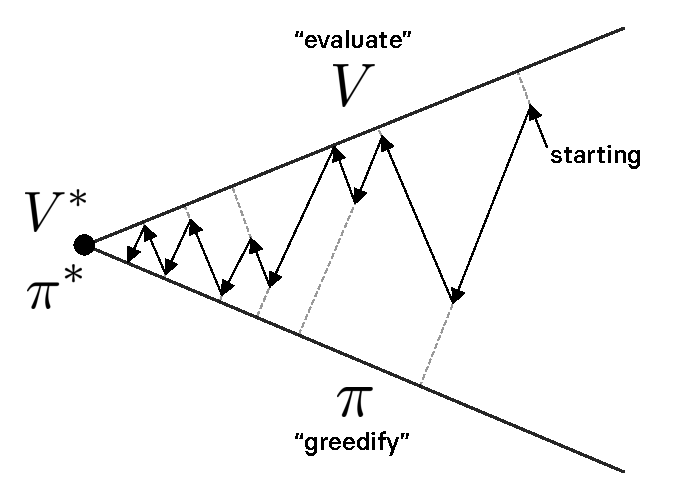
\includegraphics{Diags/gpi}}
\caption{Sequence diagram representation of generalized policy iteration (GPI)
--- similar to the one in \cite{Sutton1998-ow}, except that
the consecutive policy evaluation and improvement sub-goals are not performed to completion at each step.
$V$ and $Q$ can be used interchangeably; the principle remains intact.}
\label{fig:gpi}
\end{figure}

To get a better grasp of how entangled the objectives optimized by $Q_\omega$ and $\pi_\theta$
are in effect, we here denote their respective losses in the GPI procedure by $\ell_\omega^\textsc{td}$
and $\ell_\theta$.
These losses write as follows:
\begin{align}
\ell_\omega^\textsc{td}
\coloneqq
\widehat{\mathbb{E}}_{s_t,a_t,r_t,s_{t+1}}
\Bigg[
\bigg(
Q_\omega(s_t,a_t) -
\Big(r_t + \mathbb{E}_{a' \sim \pi_\theta(\cdot|s_{t+1})}
\big[
Q_\omega(s_{t+1},a')
\big]
\Big)
\bigg)^2
\Bigg]
\label{intro:gpiomegatd}
\end{align}
\begin{align}
\ell_\theta
\coloneqq
- \widehat{\mathbb{E}}_{s_t}
\Big[
\mathbb{E}_{a \sim \pi_\theta(\cdot|s_t)}
\big[
Q_\omega(s_t,a)
\big]
\Big]
\label{intro:gpitheta}
\end{align}
where $\widehat{\mathbb{E}}_{s_t,a_t,r_t,s_{t+1}}$ (and $\widehat{\mathbb{E}}_{s_t}$)
signify that the expectation is taken over
the effective distribution according to which the transitions $(s_t,a_t,r_t,s_{t+1})$ (and states $s_t$,
respectively) are distributed. These samples may come from various sources, whose nature determines
whether the method is online or offline, and whether it is on-policy or off-policy.
Albeit out of scope for the currently followed line of reasoning, we revisit GPI in the \emph{offline} RL
setting through an in-depth and in-breadth study in \textsc{Chapter}~\ref{thesis:chap3}.

Note, in GPI, the value function $Q_\omega$ need not be learned via TD learning
(\textit{cf.}~\textsc{eq}~\ref{intro:gpiomegatd}),
it can also be \emph{fitted}
directly in a standard supervised fashion to a Monte-Carlo estimation of the value.
$\ell_\omega^\textsc{mc}$ writes:
\begin{align}
\ell_\omega^\textsc{mc}
\coloneqq
\widehat{\mathbb{E}}_{s_t,a_t,r_t,s_{t+1}, \ldots}
\bigg[
\Big(
Q_\omega(s_t,a_t) -
\mathbb{E}_{\pi_\theta}^{> t} \big[R_t^\gamma\big]
\Big)^2
\bigg]
\label{intro:gpiomegamc}
\end{align}
where the syntactic sugar $\mathbb{E}_{\pi_\theta}^{> t} [\cdot]$ signifies that the expectation of $R_t^\gamma$
(defined in line with \textsc{eq}~\ref{intro:returndef}) is taken
\textit{w.r.t.} every possible outcome ensuing from picking action $a_t$ in state $s_t$
and following $\pi_\theta$ thereafter
in the MDP.
Note, the notation used in \textsc{eq}~\ref{intro:valuedef} was $\mathbb{E}_{\pi}^{\geq t} [\cdot]$,
which did also take the expectation over the actions done at state $s_t$ because it corresponded to
the definition of $V^\pi$. By contrast, we are here handling \emph{action}-values, which
do not contain an expectation over the current action choice.
Lastly for \textsc{eq}~\ref{intro:gpiomegamc},
$\widehat{\mathbb{E}}_{s_t,a_t,r_t,s_{t+1}, \ldots}$ signifies that, to carry out the learning update,
the agent must have access to the episode segment starting from stage $t$ and ending at episode termination.
In practice, the agent must wait until the episode is over, compute the empirical discounted sum of reward
from $t$ to termination, and use this quantity as MC target for $Q_\omega$ at $(s_t,a_t)$.
One clear advantage of TD over MC is then that TD learning need not wait for the episode to terminate to
be able to learn from the acquired samples.
This is because TD learning \emph{bootstraps} the value estimate at the current state with the value estimate
at the subsequent state, in effect \textit{``learning a guess from a guess''} (\textit{cf.}~\cite{Sutton1998-ow}).
As such, despite being being able to perform updates from incomplete trajectories (allowing for better
sample-efficiency), the TD learning objective in \textsc{eq}~\ref{intro:gpiomegatd} is inherently
less stable and tedious to tame than the MC-based objective in \textsc{eq}~\ref{intro:gpiomegamc}.
It is then not surprising that tricks like target networks --- allowing the agent to mitigate
the non-stationarity of the bootstrapped target --- proved crucial empirically.

The crux of GPI and what \textsc{Figure}~\ref{fig:gpi} illustrates is that if both processes
(policy improvement and evaluation) stabilize,
\textit{i.e.} stagnate as the alternation keeps on being carried out, then the value function
and the policy \emph{must} be \emph{jointly} optimal.
Note, if the policy is almost perfectly greedy \textit{w.r.t.} the value,
the inner expectation $\mathbb{E}_{a' \sim \pi_\theta(\cdot|s_{t+1})}[Q_\omega(s_{t+1},a')]$
that appears in \textsc{eq}~\ref{intro:gpiomegatd}
is approximately equal
to $\max_{\tilde{a} \in \mathcal{A}} \, Q_\omega(s_{t+1},\tilde{a})$,
itself appearing in \textsc{eq}~\ref{intro:tderrorloss} (omitting here the target network use for symmetry).
By training the value to be consistent \textit{w.r.t} (equivalently, to evaluate) such a policy
according to \textsc{eq}~\ref{intro:gpiomegatd},
one is therefore essentially urging the value to be the solution of the optimality version of Bellman's equation
(via TD error minimization).
As such, as soon as the policy is close to optimal, the value is trained to align with the
(unique; discussed earlier) optimal value.
Conversely, as soom as the value is close to optimal, acting greedily \textit{w.r.t} naturally defines
\emph{an} (\textit{a priori} non-unique; discussed earlier) optimal policy.
This discussion should not be held as rigorous proof of why GPI enables both policy and value to
converge to their optimal counterparts
--- proof based on the \textit{policy improvement theorem}, reported \textit{e.g.} in \cite{Sutton1998-ow}.
Instead, it provides an intuitive depiction of how the interactive
alternation of improvement and evaluation steps
\emph{cooperatively} moves the policy and value towards reaching a status of \emph{shared} optimality
they will ultimately reach together at the limit,
while being functionally unable to achieve their common goal on their own
(\textit{cf.} their objectives in \textsc{eq}~\ref{intro:gpiomegatd} and \textsc{eq}~\ref{intro:gpitheta},
displaying how they can \emph{not} function in individually in isolation).
Policy improvement and evaluation could also be seen as \emph{competing} processes:
\textit{a)} when the policy changes, the value is not consistent \textit{w.r.t} it, and
\textit{b)} when the value changes, the policy is not greedy \textit{w.r.t} it anymore.

In order to optimize the decision rule followed by the agent encoded by the policy $\pi_\theta$,
the gradient of its objective, laid out in \textsc{eq}~\ref{intro:gpitheta}, must be computer
(gradient-based optimization dealt with earlier).
Computing and taking a step along the gradient of $\ell_\theta$ \textit{w.r.t} the parameter vector $\theta$
to optimize the policy via a gradient-based optimizer defines a spawns an entire class of algorithms
called \emph{policy-gradient} algorithms (\textit{cf.} \cite{Sutton1999-ii} for their inception,
and \cite{Sutton2001-vh} where Sutton compares an array of policy-gradient algorithms).
If TD learning is used to learn $Q_\omega$ in GPI, \textit{i.e.} if $Q_\omega$ is updated
to optimize \textsc{eq}~\ref{intro:gpiomegatd},
then the resulting method is known as an \emph{actor-critic},
where $\pi_\theta$ is the actor, and $Q_\omega$ is the critic (as it evaluates, or \emph{critiques}, $\pi_\theta$).
These methods are described in \cite{Sutton1998-ow} (\textsc{Chapter}~13.5).
As such, actor-critic architectures are \textit{a fortiori} a subclass of policy-gradient algorithm.
Historically,
the first notable occurrences of actor-critics in the policy-gradient research landscape were
\cite{Konda2000-ef,Peters2005-ve,Bhatnagar2007-bz,Peters2008-mw,Degris2012-qd},
tackling the on-policy setting.
The first off-policy actor-critic algorithm and companion \textit{Off-policy Policy-gradient Theorem}
were developed by Degris in \cite{Degris2012-gv}, dealing with stochastic policies.
Specific variants of the on-policy and off-policy policy-gradient algorithms
were then developed by Silver
in \cite{Silver2014-dk} for deterministic policies.
Their main contribution is the \textit{Deterministic Policy-gradient Theorem},
and is instrumental in both algorithms (on- and off-policy one).

All in all, a large majority of RL algorithms
aiming to learn the optimal control in the sense of Bellman
\emph{can} be framed under
the unifying GPI framework, with an identifiable learned policy and value.

Another type of approach, spawning the class of \textit{likelihood-ratio} policy-gradient algorithms,
does not learn a critic in its bare-bones form, just a policy $\pi_\theta$.
To get a gradient to update $\pi_\theta$,
it computes the \emph{real} Monte-Carlo return
and use this raw estimate of the value instead of $Q_\omega$
as it is currently laid out in \textsc{eq}~\ref{intro:gpitheta}.
Since the back-propagation of gradients can not occur through this raw estimate,
these methods rely on the \emph{score function gradient estimator} trick to estimate the gradient.
This trick transforms the initially pathological gradient into
the gradient of the logarithm of $\pi_\theta$, weighted by the effective MC return, per action choice.
In essence, the problem is reduced to a return-weighted $\log$-likelihood maximization problem,
which increases the probably for the agent of performing a certain action if the effective return of that action
is high. The higher the return, the more this gradient estimate pushes up the $\log$-probability of the action that
led to this return (\textit{e.g.} REINFORCE \cite{Williams1992-xn},
often used across ML disciplines to from gradients from non-differentiable losses and \textit{black-boxes}).
